
\section{Sotwares developed}

\section{TCGAbiolinks: An R package to download and analyze data from TCGA}


 Integrative analysis of genomic big-data collections from public databases such as The Cancer Genome Atlas (TCGA) can advance knowledge and lead to new discoveries in cancer research.  However, the data retrieval from TCGA is a cumbersome and time-consuming task. The TCGABiolinks Bioconductor package allows to query, download and perform integrative analysis with TCGA data, combining computer science and statistical methods thus authoring reproducible analysis. 
  Case studies are reported on various cancer system biology applications including a complete downstream analysis with LGG and GBM, by means of gene expression data,  methylation data and integration of both data.
  The analysis layer and visualization layer were combined into a reusable workflow. 
  The TCGABiolinks package is released under GPL3 License within Bioconductor project. The source code and vignette are freely available at \url{http://bioconductor.org/packages/TCGAbiolinks/}.
  
  The Cancer Genome Atlas (TCGA) has made the effort to collect a wide range of different data sets and at the same time offers an API to access these data sets. However, this can only be seen as the first step towards allowing different researchers access to these data sets. The question that needs to be answered next is how can we best access, prepare and then analyze the data most efficiently given a specific problem. 
The number of publications in pubmed related to TCGA (July 2015) is 1517 and the number of publications per year has increased every year since its conception (Figure~\ref{NAR-fig1}).

\begin{figure}
\centering
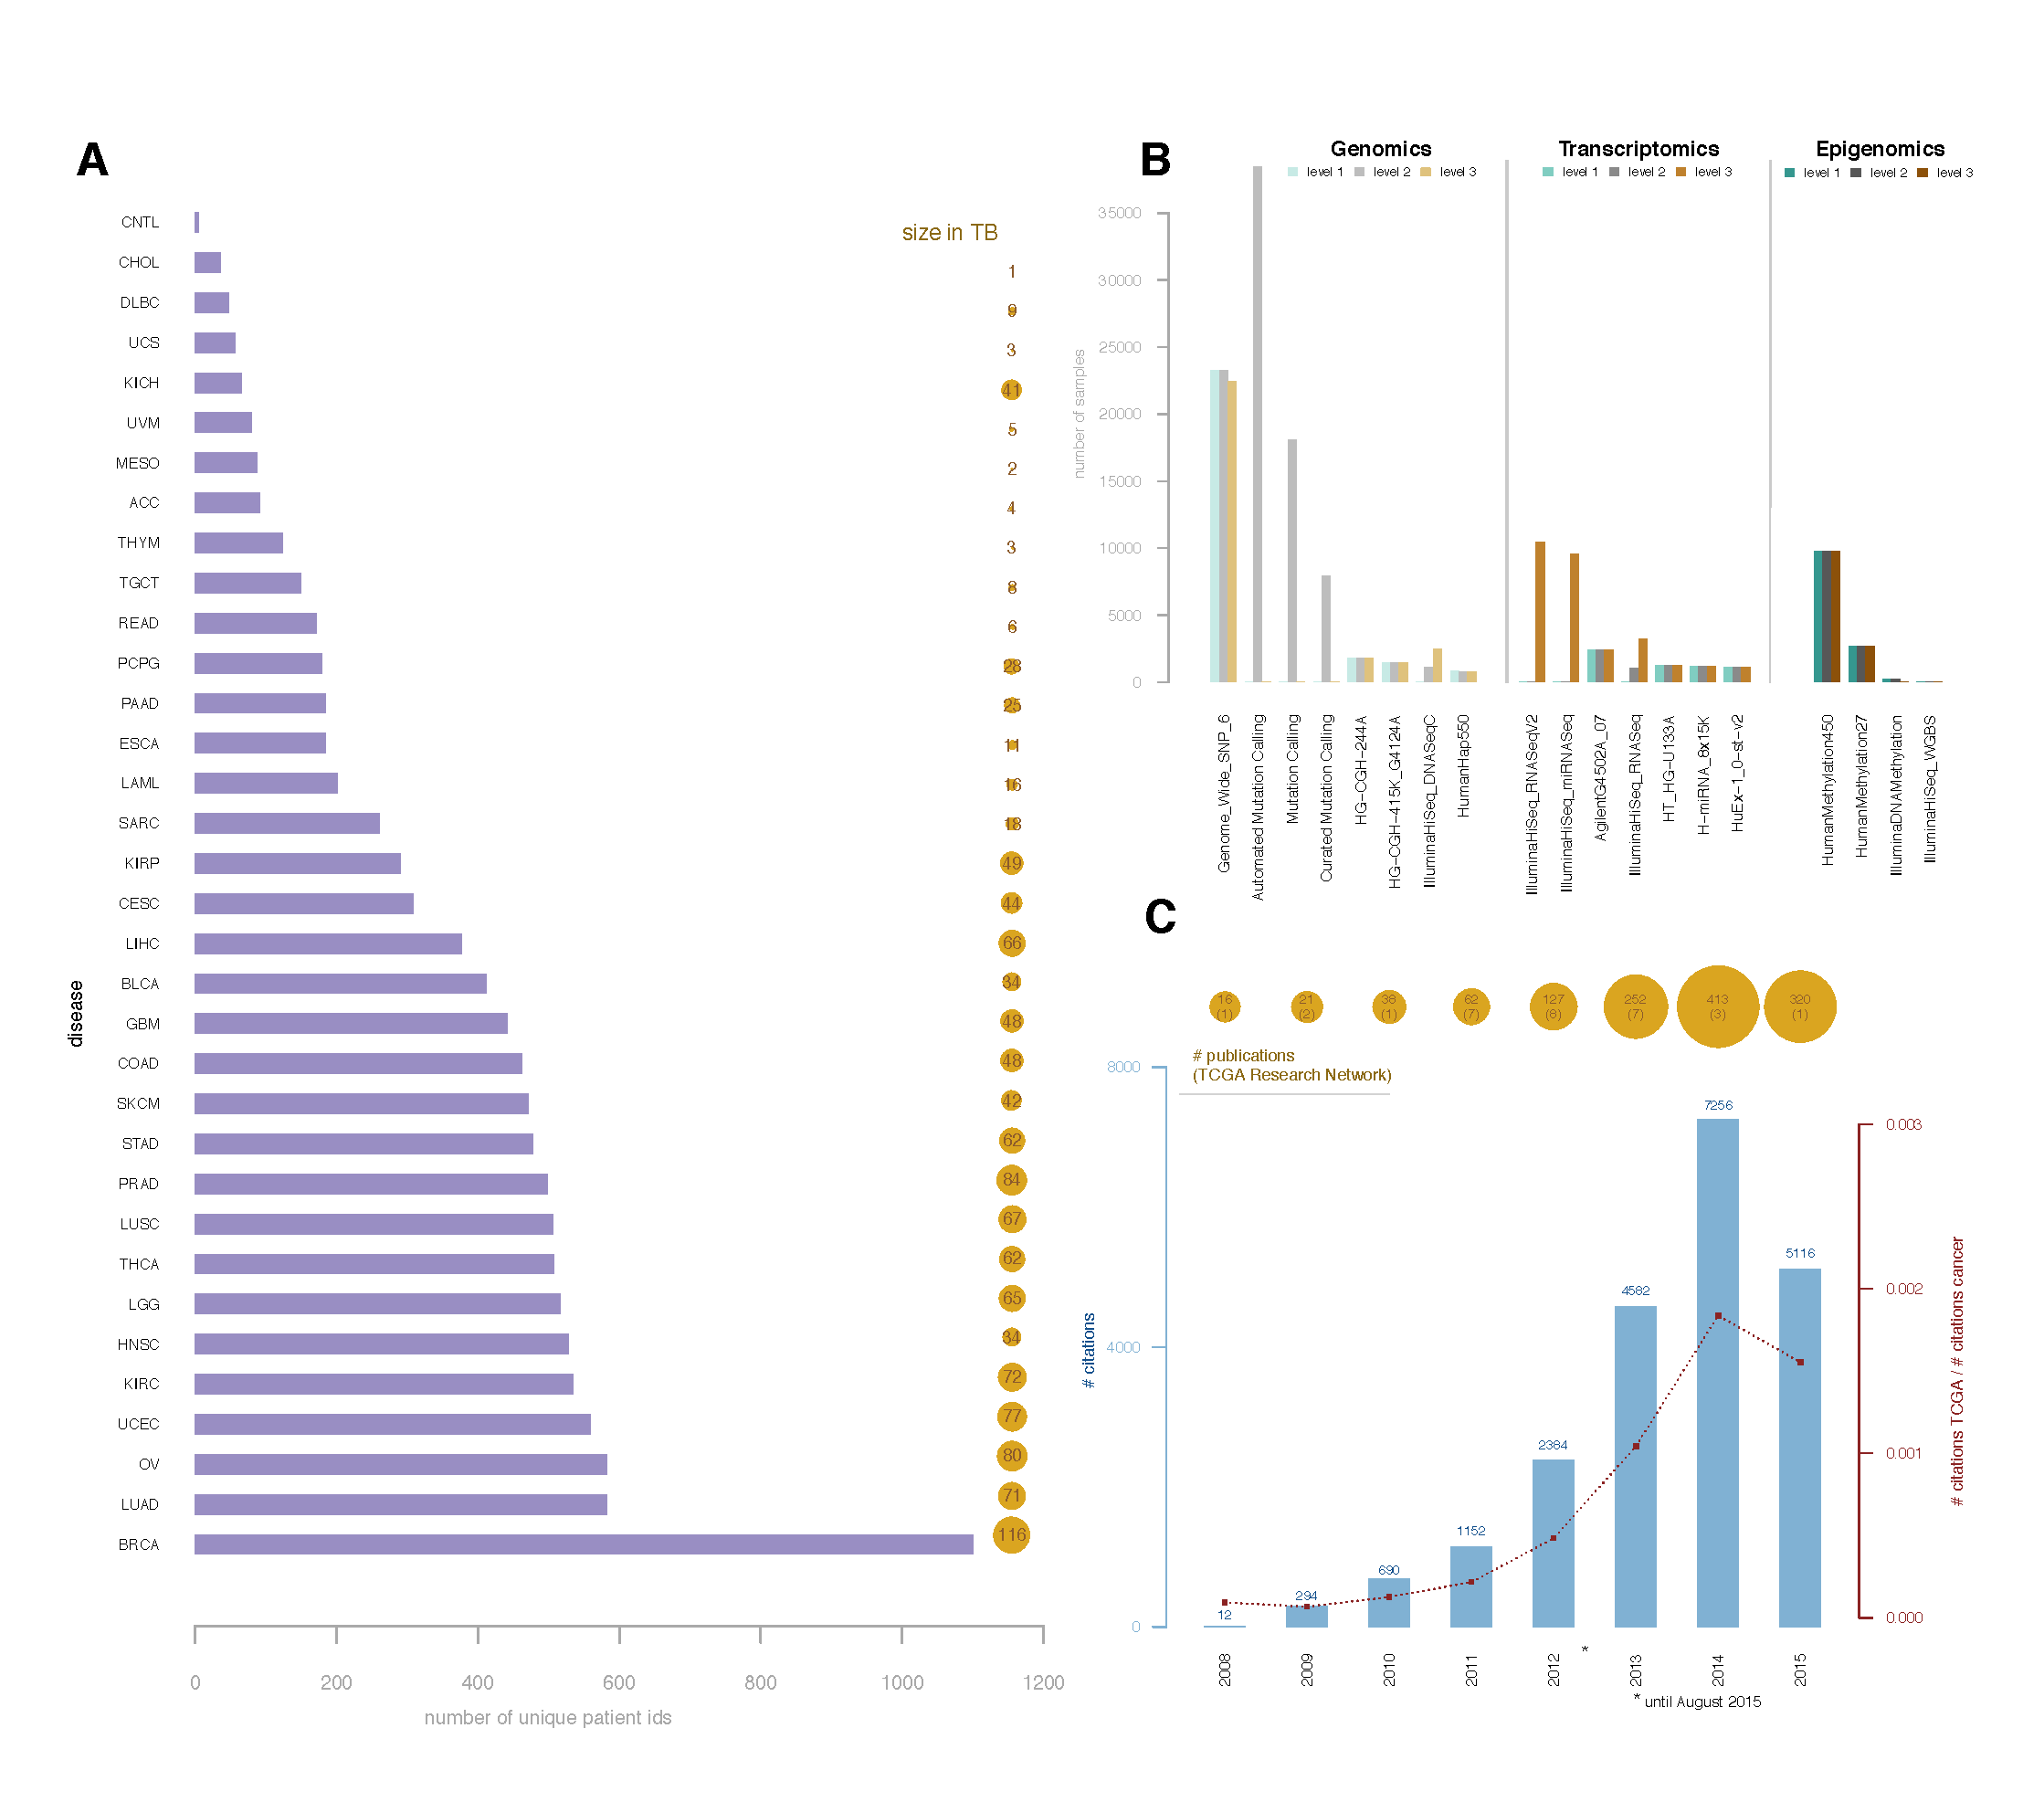
\includegraphics[width=1.0\textwidth]{images/figure1_draft2.pdf}
\caption{\textbf{A}: bars represent number of patients by disease, bubbles represent the available data size in TB by disease; \textbf{B}: number of samples by platform and by level, grouped by type: genomic, transcriptomic and epigenomic; \textbf{C}: number of citations for TCGA papers and number of these papers by year in bubbles (left y-axis), in parentheses the number of papers published by the TCGA Research Network; red dots and line: quotient number of TCGA papers/number of cancer papers (right y-axis) , source Scopus searches "TCGA" with parameter "All Fields" and search "cancer" with parameter "All Fields" (adding TCGA Research Network papers that were not found during this search)}
\label{fig:my_label}
\end{figure}

This increased publication frequency does not only imply that the number of researchers that use TCGA data increases but it also attracts researchers new to these data sets.
There are two distinct groups of researchers such as beginners-intermediate and advanced and they are very different in nature. 
While the former still spends a large amount of time on downloading and pre-processing the data for the subsequent analyses, the latter first has to understand both the different data types and the analyses typically applied to them. The usual approach for obtaining help for both types of users consists in asking questions on portals such as \textit{stackoverflow.com}, \textit{support.bioconductor.org} or \textit{biostars.org}.\\

%%%%%%%%% Reduce state of art in one paragraph %%%%%%%%% 

Recently, different tools to retrieve TCGA datasets have been made available, these include TCGA-Assembler  (\cite{Zhu14}), CGDS-R (\cite {gao2013integrative}), cBioPortal \cite{cerami2012cbio}, canEnvolve (\cite{samur2013canevolve}), BioXpress \cite{wan2015bioxpress},  Firehose \footnote{http://gdac.broadinstitute.org}, and
RTCGAtoolbox~\cite{samur2014rtcgatoolbox}.
% Reorganize the features in 3 categories
The features for each tool can be divided into four representative categories (i) downloader, ii) data integration and analysis, and iv) visualization. 
The fist category comprises tools that mainly download cancer genomics data: TCGA-Assembler, the Bioconductor package CGDS-R and cBioPortal. 
% TCGA-Assembler written in R apply a recursive algorithm to retrieve the URLs of all data files. This open software package automates and streamlines the acquisition, assembling, and processing of public TCGA data. It can be integrate with R libraries for downstream analysis.
% CGDS-R, at the moment, the only tool available on CRAN or Bioconductor provides a basic set of R functions for querying the Cancer Genomic Data Server (CGDS) hosted by the Computational Biology Center (cBio).
% cBioPortal is a web portal for interactively exploring multidimensional cancer genomics data sets in the context of clinical data and biologic pathways. It allows explorative data analysis, and provides simple download of small data slices.
% A key feature of the cBio portal is ease of use, if you want to explore a pathway of interest in one or more cancer types, but to download raw mRNA expression files or full segmented copy number files, it's not suitable.
The second category includes tools that focus on data analysis and integration, such as Firehose, canEnvolve or BioXpress.
% canEnvolve contains integrated data from 90 studies involving more than 10000 patients. Data analysis are involved at different levels: 1) mRNA/miRNA and copy number 2) integrative analysis between genes, protein and copy number 3) network and pathway analysis 4) survival analysis. It is a web portal and can be a limit for researchers that want to analyse data in an R environment. \\
% BioXpress \cite{wan2015bioxpress} database stores RNA-seq data from several publicly available sources, among them TCGA, and through standardize method identifies the expression levels of the genes. 
% The third category includes tools to download, analyse, and integration data, such as Firehose.
% The Firehose has been developed to download and analyze (e.g. GISTIC 2.0 and MutSig), in an automated and reproducible way, the data generated by TCGA. The results are  available via a website.  However, it has several limitations to access the data and it is not easily integrated with programming environments for downstream analysis(\cite{samur2014rtcgatoolbox}). \\
The third category comprises tools to download, analyze ,integration and visualization such as RTCGA-Toolbox.
% RTCGAToolbox (\cite{samur2014rtcgatoolbox}) was designed, using R programming language,  
to systematically access Firehose pre-processed data and to perform basic analysis and visualization.

TCGA provides unprecedented opportunities to interrogate the genome and epigenome of normal and tumor tissues proving public access to more than 20 tumor types. Markedly however, preparing these data for various  analysis pipelines 
is a time-consuming task as the biological information is stored in different formats through a large number of files.

Despite the existence of some integrative TCGA-specific software packages, few are available from Bioconductor and none or few of them perform integrative analysis. 
Being part of the Bioconductor project ensures the high-quality, well documented and interoperable software and the possibility of integration with hundreds of available packages.
%,  helping the user to work with different packages and analysis.


We introduce \textit{TCGAbiolinks} an R/Bioconductor package for integrative analysis with TCGA data.
The aim of TCGAbiolinks is four-fold: i) facilitate the data retrieval, ii) prepare the data using the appropriate pre-processing strategies, iii) provide the means to carry out different standard analyses and iv) allow the user to download a specific version of the data and thus to easily reproduce earlier research results.

In more detail, the package provides multiple methods for analysis (e.g., differential expression analysis, identifying differentially methylated regions) and methods for visualization (e.g., survival plots, starburst plots) in order to easily develop complete analysis pipelines. An example of the package overflow is presented in Figure \ref{NAR-fig3}. %flux


%%%%%%%%% NEW FIGURE

 \tikzstyle{texto} = [above, 
 					  text width=6em, 
                      text centered,
                      font=\normalsize]

\tikzstyle{start} = [rectangle,
                     minimum size=6mm,%rounded corners=3mm,
					 very thick,
                     draw = black!50, 
                     top color = white,
                     bottom color = black!20,
                     font=\itshape\footnotesize,
                     drop shadow, 
                     align=center]
                     
\tikzstyle{fail} = [rectangle, 
					rounded corners, 
                    minimum width=3cm, 
                    minimum height=1cm,
                    text centered,
                    font=\itshape\footnotesize, 
                    draw=black, 
                    fill=red, 
                    text=white,  
                    drop shadow]
                    
\tikzstyle{success} = [rectangle, 
					   rounded corners, 
                       minimum width=3cm, 
                       font=\itshape\footnotesize,
                       minimum height=1cm,
                       text centered, 
                       draw=black,
                       fill=green!70!black!70, 
                       text=white,  
                       drop shadow]
\tikzstyle{process} = [rectangle, 
					   minimum width=1cm, 
                       minimum height=0.5cm, 
                       text centered, 
                       text width=3cm, 
                       font=\itshape\footnotesize,
                       draw=black, 
                       fill=black!40, 
                       text=white,drop shadow]
\tikzstyle{decision} = [diamond, 
						minimum width=0.5cm, 
                        minimum height=0.5cm,
                        font=\itshape\footnotesize,
						text centered, 
                        draw=black,
						top color = white,
                        bottom color = yellow!80, 
                        text=black, 
                        drop shadow]
                        
\tikzstyle{arrow} = [thick,->,>=stealth,-latex',draw,rounded corners]
\tikzstyle{cloud} = [draw, 
					 ellipse,
					 rounded corners = 3mm,
                     very thick,
                     draw           = orange!50, 
                     top color      = white,
                     bottom color   = orange!20,
                     font           = \itshape\footnotesize,
                     node distance  = 4cm,
                     minimum height = 1em,
                     drop shadow]


\begin{figure}[!h]
 \begin{center}
 \begin{tikzpicture}[node distance = 1.5cm, 
 					 auto, shorten >=1pt,
                     thick,font=\itshape\footnotesize,
                     ->,
                     >=stealth']
 \linespread{0.8}{

 \node (clinic) [start]{TCGAquery\_clinic};
 \node (start) [start, below of=clinic,yshift=0.5cm] {TCGAquery};
 \node (download) [start, below of=start,yshift=0.5cm] {TCGAdownload};
 \node (prepare) [start, below of=download,yshift=0.5cm] {TCGAprepare};
 \node (version) [start, below of=prepare,yshift=0.5cm] { TCGAquery\_version};

 \node (coxnet) [start, right of=clinic, yshift=0cm,xshift = +1.5cm] {survivalCoxNET};
 \node (survival) [start, right of=start, yshift=0cm,xshift = +1.5cm] {survival};
 \node (eacomplete) [start, right of=download, yshift = 0cm,xshift = +1.5cm] {EAcomplete};
 \node (eabarplot) [start, right of=eacomplete, xshift = +1cm] {EAbarplot};
 \node (dea) [start, right of=prepare,yshift = 0cm, xshift = +1.5cm] {DEA};
 \node (dmr) [start, right of=version, xshift = +1.5cm,yshift = 0cm] {DMR};

 \node (starburst) [start, right of=dmr, xshift = 1cm,yshift = 0.3cm] {starburst};

 \tikzstyle{texto} = [above, text width=6em, text centered,font=\normalsize]

 \path [arrow] (start) -- (download);
 \path [arrow] (download) -- (prepare);
 \path [arrow] (prepare) -- (eacomplete);
 \path [arrow] (eacomplete) -- (eabarplot);
 \path [arrow] (prepare) -- (dea);
 \path [arrow] (prepare) -- (dmr);
 \path [arrow] (dmr) -- (starburst);
 \path [arrow] (dea) -- (starburst);
 \draw (prepare) edge[out=0,in=180,->,color=red!80!black] (dmr);
 \draw (prepare) edge[out=0,in=180,->,color=green!60!black] (dea);
 \draw (prepare) edge[out=0,in=200,->,color=green!60!black] (eacomplete);
 \draw (prepare) edge[out=0,in=180,->,color=green!60!black] (coxnet);
 \draw (clinic) edge[out=0,in=180,->,color=blue!80!black] (coxnet);
 \draw (clinic) edge[out=0,in=180,->,color=blue!80!black] (survival);
 \path [arrow,color=blue!80!black] (clinic) -- (survival);

 }
 % Background
 \begin{pgfonlayer}{background}
   \begin{pgfonlayer}{background}
         % Compute a few helper coordinates
         \path (start.west |- start.north)+(-0.5,0.5) node (a) {};
		 \path (prepare.south -| prepare.east)+(+0.3,-0.2) node (b) {};
		 \path (clinic.west |- clinic.north)+(-0.5,0.6) node (a) {};
         \path (dmr.south -| prepare.east)+(+0.3,-0.2) node (b) {};
         \path (starburst.south -| eabarplot.east)+(+0.25,-0.55) node (c) {};
         \path (eabarplot.west |- survival.north)+(-0.2,1.65) node (d) {};
		 \path (dmr.south -| coxnet.east)+(+0.2,-0.225) node (e) {};
         \path (coxnet.west |- survival.north)+(-0.2,1.65) node (f) {};
         \path[fill=cyan!20,rounded corners, draw=black!50, dashed]
             (a) rectangle (b);
         \path (dmr.west |- clinic.north)+(-0.2,1.0) node (a) {};
         \path (dmr.south -| starburst.east)+(+0.2,-0.3) node (b) {};
         \path[fill = yellow!30,
               rounded corners, 
         	   draw = black!50, dashed]
             (e) rectangle (f);
         \path (clinic.west |- clinic.north)+(0.65,0.3) node (u1)[texto,font=\normalsize]
       {\normalsize{Data functions}};
         \path (survival.north |- dmr.east)+(+0.0,+4.65) node (u1)[texto,font=\normalsize] {\normalsize{Analysis}};
          \path[fill = magenta!20,
                rounded corners, 
                draw = black!50, 
                dashed]
            (d) rectangle (c);
         \path (starburst.north |- starburst.east)+(-0.1,+4.35) node (u1)[texto,font=\normalsize] {\normalsize{Visualize}};
 	\end{pgfonlayer}
 \end{pgfonlayer}

 \end{tikzpicture}
 \end{center}
 \caption[Example of TCGAbiolinks workflow]{Example of a complete workflow using TCGAbiolinks: functions were divided in three groups - data (blue), analysis (yellow) and visualize (green). Green arrows represent expression data, red arrows methylation data and blue arrows clinical data. The function TCGAquery searches for TCGA data using as input the tumor type, platform, level, version of the data and list of samples. The output of TCGAquery will be downloaded with TCGAdownload. TCGAprepare will read the data and prepare the data into a SummarizedExperiment object.%, if save parameter is true the final object is saved. 
 Afterwards, downstream analyses can be performed. For example for methylation data, TCGAanalyze\underline{\space}DMR can be used for Differential methylation analysis. Differential expression analysis can be carried out with TCGAanalyze\_DEA. Integrative visualization of  both results  is possible  using TCGAvisualize\underline{\space}starburst.} 
 \label{NAR-fig3} %flux
 \end{figure}




\section{MATERIALS AND METHODS}
\subsection{The TCGAbiolinks package}

\textit{TCGAbiolinks} is composed of seven functions / layers that can be grouped into three levels: DATA, APPLICATION and SOCIAL.
%This idea was inspired to Open Systems Interconnection model (OSI Model) ISO/OSI layers, and like ISO OSI the data passes severals levels from TCGA ftp folders, where TCGA's data are located, to application level. Furthermore we added a social level more.
These functions can be used independently but also in combination to provide the user with fully understandable analysis pipelines applied to TCGA data.

%\begin{itemize}
%\item DATA: \textit{TCGAquery}, \textit{TCGAdownload}, \textit{TCGAprepare}
%\item APPLICATION: TCGAanalyze, TCGAvisualize
%\item SOCIAL: TCGAinvestigate, TCGASocial
%\end{itemize}

%\begin{figure}[!h]
%\begin{center}
%\includegraphics[width=.9\linewidth]{images/TCGAbiolinks_levels.png}
%\includegraphics[width=.9\linewidth]{images/TCGAbiolinks_levels2.png}
%\end{center}
%\caption{TCGAbiolinks layered functions levels}
%\label{NAR-fig2}
%\end{figure}


\subsection{Outline of the TCGAbiolinks package functionalities.}
\begin{figure*}
\centering
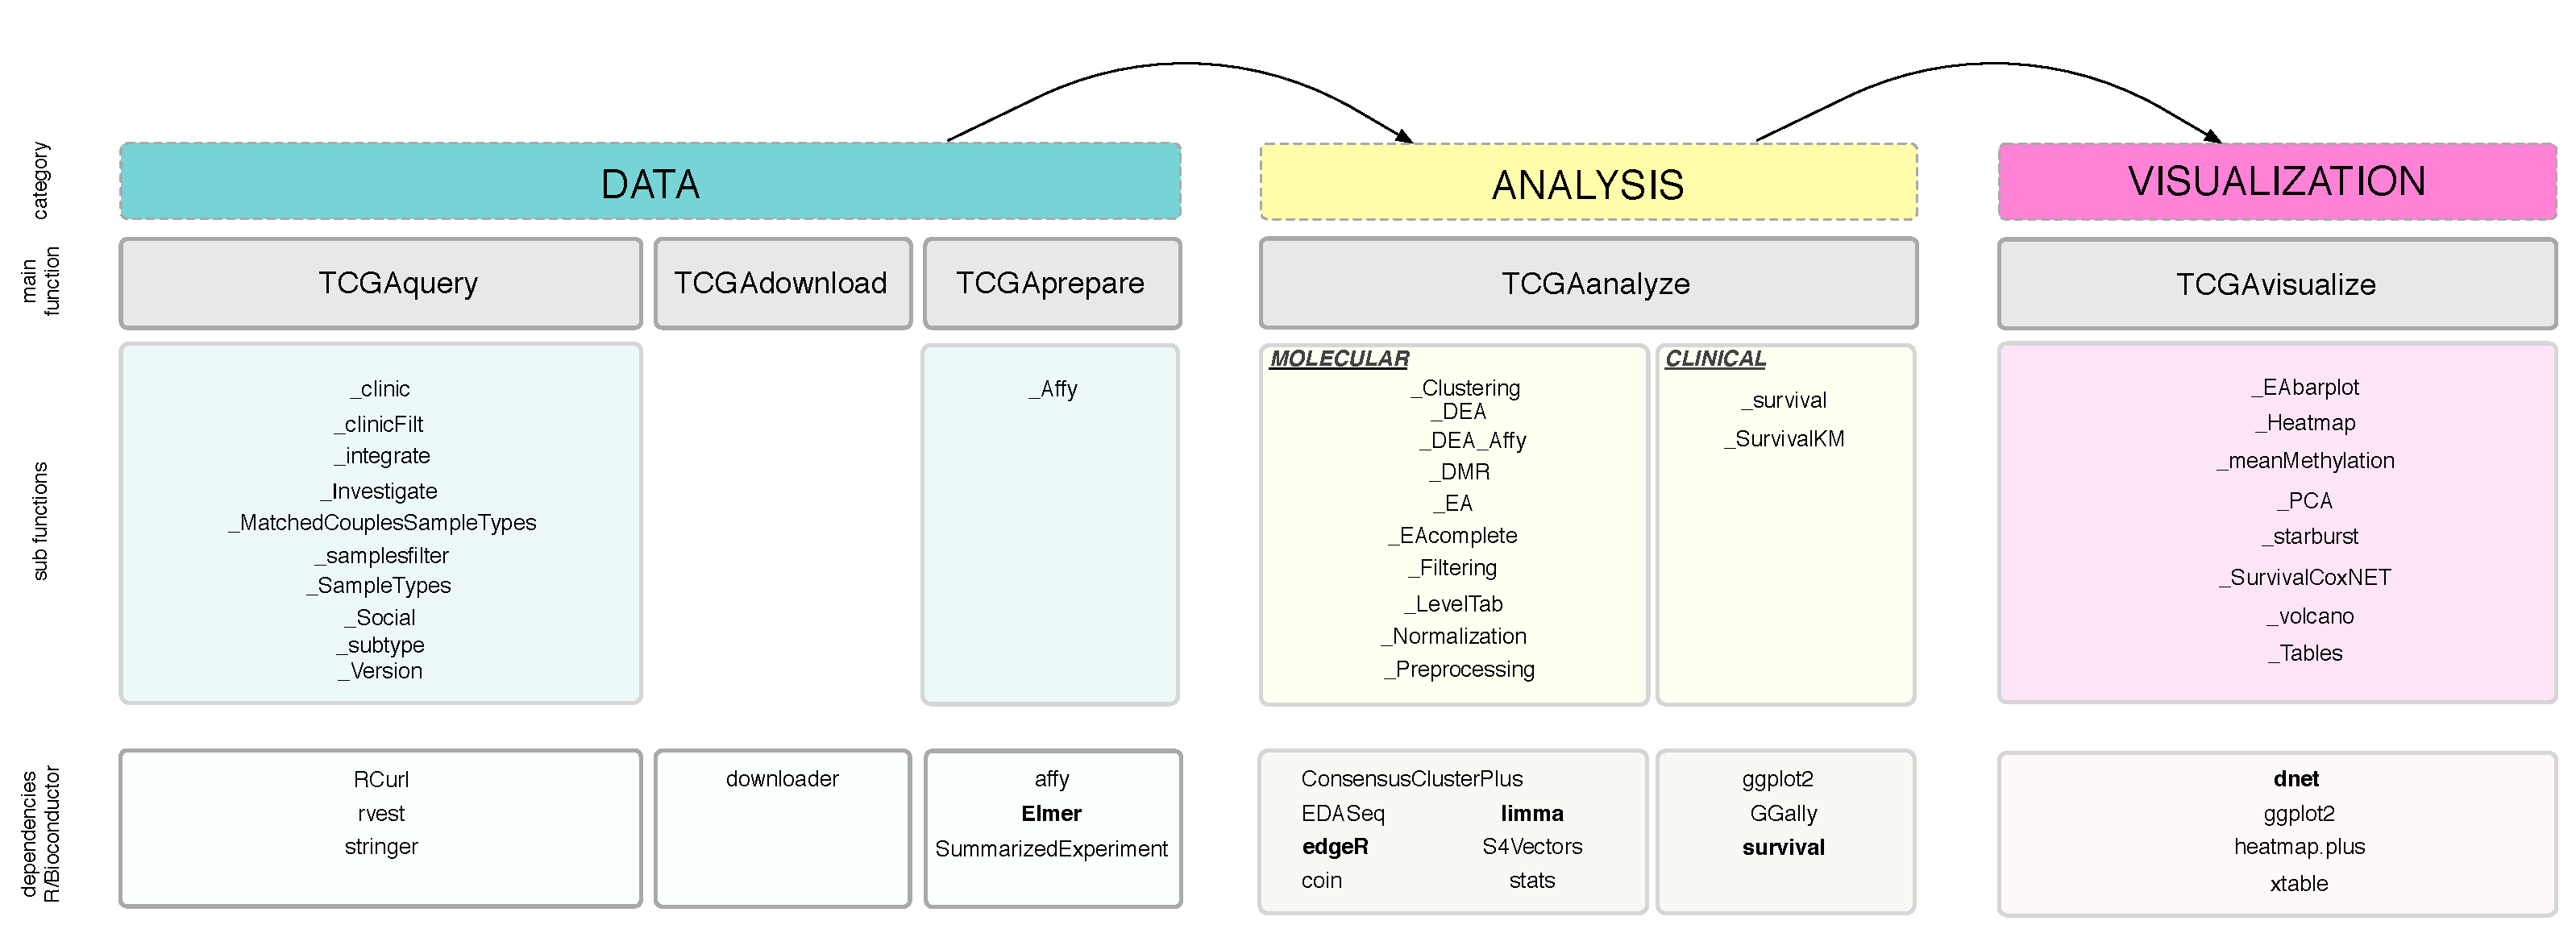
\includegraphics[width=\textwidth]{images/workflow_draft2_noboxes.pdf}
\caption{TCGAbiolinks is organized in three categories. In the first category (DATA), functions to query the TCGA database, to download the data and to prepare it are made available. The second category (ANALYSIS) contains functions that allow the user to carry out different types of analyses, these incluse clustering (TCGAanalyze\_Clustering), differential expression analysis (TCGAanalyze\_DEA) and enrichment analysis (TCGAanalyze\_EA). Finally, the obtained results can be visualized using the functions in the third category (VISUALIZATION): these include principal component analysis (TCGAvisualize\_PCA), starburst plots (TCGAvisualize\_starburst) and survival curved (TCGAvisualize\_SurvivalCoxNET). The different dependencies to other R/Bioconductor packages are named in the last row of the figure.}
\label{fig:workflow}
\end{figure*}
%With our new R package, called \textit{TCGAbiolinks}, we proposed some solutions for bioinformaticians to save their (researcher and computational) time, trying  to address the needs of both groups as follows.
%See TCGAbiolinks Bioconductor user’s guide for a more detailed description.

TCGAbiolinks simplifies access, preparation and downstream analysis of cancer data by providing high-level functions
which warp different packages as reported in the table below:  
%In the following table we reported the functions for each layer and related package used / wrapping.

% \begin{table}[ht]
% \centering
% \begin{tiny}
% \begin{tabular}{lll}
% \hline
% Layer & Function & Package used (wrapping)  \\ 
% \hline
% \cellcolor{cyan}query & TCGAquery\_clinic & RCurl \\ 
% \cellcolor{cyan}query & TCGAquery\_clinicFilt & \\ 
% \cellcolor{cyan}query & TCGAquery\_integrate & \\ 
% \cellcolor{cyan}query & TCGAquery\_MatchedCoupledSampleTypes & \\ 
% \cellcolor{cyan}query & TCGAquery\_samplesfilter & \\ 
% \cellcolor{cyan}query & TCGAquery\_SampleTypes RCurl & \\ 
% \cellcolor{cyan}query & TCGAquery\_Version & rvest, stringr \\ 
% \cellcolor{cyan}query & TCGAquery & downloader\\ 
% & & \\
% \cellcolor{yellow}download & TCGAdownload & \\ 
% & & \\
% \cellcolor{brightgreen}prepare & TCGAprepare & SummarizedExperiment, Elmer \\ 
% & & \\
% \cellcolor{coolgrey}analyze & TCGAanalyze\_DEA & edgeR\\ 
% \cellcolor{coolgrey}analyze & TCGAanalyze\_DMR & ggplot2, SummarizedExperiment,S4Vectors \\ 
% \cellcolor{coolgrey}analyze & TCGAanalyze\_EA & stats &\\ 
% \cellcolor{coolgrey}analyze & TCGAanalyze\_EAcomplete &\\ 
% \cellcolor{coolgrey}analyze & TCGAanalyze\_Filtering &\\ 
% \cellcolor{coolgrey}analyze & TCGAanalyze\_LevelTab & \\ 
% \cellcolor{coolgrey}analyze & TCGAanalyze\_Normalization & EDASeq\\ 
% \cellcolor{coolgrey}analyze & TCGAanalyze\_Preprocessing & grDevices \\ 
% \cellcolor{coolgrey}analyze & TCGAanalyze\_survival & GGally,survival,scales  \\ 
% \cellcolor{coolgrey}analyze & TCGAanalyze\_SurvivalKM & survival \\ 
% & & \\
% \cellcolor{darkorange}visualize & TCGAvisualize\_EAbarplot & \\ 
% \cellcolor{darkorange}visualize & TCGAvisualize\_meanMethylation & ggplot2, SummarizedExperiment\\ 
% \cellcolor{darkorange}visualize & TCGAvisualize\_PCA & \\ 
% \cellcolor{darkorange}visualize & TCGAvisualize\_starburst & \\ 
% \cellcolor{darkorange}visualize & TCGAvisualize\_SurvivalCoxNET & dnet\\ 
% & & \\
% \cellcolor{red}investigate & TCGAinvestigate & RCurl\\ 
% & & \\
% \cellcolor{bleudefrance}social & TCGAsocial & \\

% \hline
% \end{tabular}
% \end{tiny}
% \caption{TCGAbiolinks proposed functions and related wrapping packages} 
% \label{table:01}
% \end{table}

\subsection{TCGAQuery}

This functions is the core of the package that allows user to query data from the TCGA portal. 
%This function allows user to query TCGA about different datatypes and different platforms.
The  TCGA portal provides data  for 24 cancer and   7 different datatypes  (clinical,  mRNA,SNP, Protein, miRNA,
Methylation, Exome) using several platform.
Data in TCGA are organized in 4 levels: 1) raw, 2) processed, 3) interpreted, and 4) region of interest. The user can access to all level, if TCGA site do not require user certification for data access.
TCGAQuery allows to programmatically interrogate the  available data in terms of:
tumor, platform, samples (barcode list), level, center and version.


%\lstinputlisting{Rcode/TCGAquery_Rscripts.R}


%\begin{lstlisting}[language=R]
%query <- TCGAquery(tumor = c("gbm","lgg"), platform=Exome)
%\end{lstlisting}

In above example we reported several example of TCGAquery functions and relative subfunctions that call TCGAquery.

will return the list of available samples with exome sequencing for the Lower Grade Glioma and Glioblastoma tumor types.
More advanced queries can be created by specifying other parameters such as level, center and others.
The return type of TCGAQuery is a list of lists, the package also provides higher level query functions (Table 1) 
which manipulate such lists. For example the TCGAquery\_clinic allows to create a table from the clinical information 

%BRCAclinic <- TCGAquery_clinic(cancer = "BRCA",clinical_data_type = "clinical_patient")

% dim(BRCAclinic)

%what gives in putput
and TCGAquery\_SampleTypes allows to filter for sample types, for example to download the list of EXOME samples of recurrent tumors for Glioblastoma

% Add an example to download Recurrent tumor of Glioblastoma GBM

%SS <- TCGAquery_SampleTypes(bar,c("TR","TRBM"))

% See table \ref{TCGAQueryoutput}

%TCGA's data are organized according datatype and platform about 24 cancers.
%In particular there are several samples with identification of TCGAbarcode
%that it is composed by 16 chrs.


%Clinical data are important because it can be used for different analysis
%like survival analysis and also to retrieve information about samples like drugs, follow up, stages, and also molecular subtypes.


\textit{TCGAquery\_clinic} 
This functions is used to query and retrieve informations about samples available in TCGA data portal see for example Fig~\ref{NAR-fig5}.

% \begin{figure}[!h]
% \begin{center}
%   \includegraphics[width=.9\linewidth]{images/clinicData2.png}
%   \end{center}
%   \caption{Example of clinical patient's data for BRCA cancer}
%   \label{NAR-fig5} % \label{fig:sfig2}
% \end{figure}

\textit{TCGAquery\_clinicFilt} 
With this function the user will filter the data, returning the list of barcodes that matches all the filter.
The information that can be retrieved are about 
\begin{tiny}
\begin{itemize}[nolistsep]
\item positive or negative her2 neu immunohistochemistry receptor status. 
\item gender, MALE or FEMALE
\item Positive or Negative Progesterone receptor status.
\item stage, Pathologic Stage: stageIX, stageI, stageIA, stageIB, stageIIX,stageIIA, stageIIB, stageIIIX,stageIIIA, stageIIIB, stageIIIC, stageIV.
\item Positive or Negative Estrogen receptor status.
\end{itemize}
\end{tiny}


\textit{TCGAquery\_samplesfilter} 
As shown in TCGAquery Rcode examples, this function help the researcher for filtering sample output from TCGAquery.

%\begin{enumerate}[topsep=0pt,itemsep=-1ex,partopsep=1ex,parsep=1ex]
\textit{TCGAquery\_integrate} 

Some times researches would like to use samples from different platforms 
from the same patient. In order to help the user to have an overview of the number of samples in commun we created this function that will receive the data frame returned from TCGAquery and produce a matrix n platforms x n platforms with the values of samples in commum.
This function creates a table with common samples analyzed with different platforms (e.g. matched miRNA-mRNA), that can be used in two by two comparison to retrieve a list of common samples (TCGA barcode) that can be downloaded saving time. 

The result of the 3 platforms for BRCA is shown below:

\begin{table}[!h]
\centering
\begin{tiny}
\begin{tabular}{llll}

  \hline
& AgilentG4502A\_07\_3 & HumanMethylation450 & IlluminaHiSeq\_RNASeqV2 \\ 
\hline
AgilentG4502A\_07\_3 & 604 & 224 & 530 \\ 
HumanMethylation450 & 224 & 930 & 790 \\ 
IlluminaHiSeq\_RNASeqV2 & 530 & 790 & 1218 \\ 
   \hline
\end{tabular}
\end{tiny}
\caption{Table common samples among platforms from TCGAquery} 
\label{table:02}
\end{table}


% We can integrate the function TCGAquery_MatchedCoupledSampleTypes in TCGAquery_SampleTypes adding some parameters and using only 1 functions for samples Types.

\textit{TCGAquery\_SampleTypes} 
This functions allows user to retreive informations about samples for example: TP, TN, etc. % add more informations
It is possible to retrieve multiple tissue types from the same patients or different one.
This function allows user to obtain a list of barcodes with a specific clinical data. For instance the user can indicate tissue type to download (primary, recurrent,metastatic,..), in case of multi tissue types can define matched sample from the same patients
\begin{table}[!h]
\centering
\begin{tiny}
\begin{tabular}{ll}
  \hline
typesample &  tissue type definition \\ 
\hline
TP &   PRIMARY SOLID TUMOR \\
TR &   RECURRENT SOLID TUMOR \\
TB &   Primary Blood Derived Cancer-Peripheral Blood \\
TRBM & Recurrent Blood Derived Cancer-Bone Marrow \\
TAP &  Additional-New Primary \\
TM &   Metastatic \\
TAM &  Additional Metastatic \\
THOC & Human Tumor Original Cells \\
TBM &  Primary Blood Derived Cancer-Bone Marrow \\
NB &   Blood Derived Normal \\
NT &   Solid Tissue Normal \\
NBC &  Buccal Cell Normal \\
NEBV & EBV Immortalized Normal \\
NBM &  Bone Marrow Normal \\
  \hline
\end{tabular}
\end{tiny}
\caption{Table with tissue type definition from TCGAquery} 
\label{table:03}
\end{table}


\subsection{TCGADownload}
TCGA's cancer data as organized in table (add) has stored on ftp site and typically and in table are reported average of size of data for each cancer and platform type.
{\color{red} Give the idea of dimension of file in GByte for each platform}
It is important the selection of only file that user need for next steps such as preparion and analysis.

The TCGAdownload function will download the data using as reference the the lines of the TCGAquery search result. 
There is an option to download the entire tar.gz folder or download specific files using the \emph{type} parameter or the \emph{samples} parameter
The output files will be saved into the path parameters. If this path does not exists the package will try to create the directories. By default, if a sample was already downloaded the function will not download again, unless the force parameter is set to \emph{TRUE}
TCGAdownload allows also to download only a list of samples as output of TCGAQuery, eg. selecting level (1,2,3) common samples between two or three platforms. 

\begin{tiny}
\begin{itemize}[nolistsep]
\item data The TCGAquery output
\item path Directory to save the downloaded data
\item type Filter the files that will be downloaded by Example:"rsem.genes.results"
\item samples List of samples to download data
\item force Download files even if it was already downladed?
\end{itemize}
\end{tiny}

\subsection{TCGAPrepare}
The TCGAPrepare function will read the data from level 3 the experiments and prepare it for downstream analysis into a SummarizedExperiment object. The samples are always refered by their barcode. If you want to save the data into an rda file, please use the \emph{save}
parameter that will save an rda object with the  \emph{filename} parameter.
If no filename was set, the filename will be the concatenation of platform and Sys.time.
You can easily read the downloaded data using the `TCGAprepare` function.
This function will prepare the data into a SummarizedExperiment

\url{http://www.nature.com/nmeth/journal/v12/n2/abs/nmeth.3252.html}
object for downstream analysis. 
For the moment this function is working only with data level 3.

The arguments are:
\begin{tiny}
\begin{itemize}[nolistsep]
\item query**	Data frame as the one returned from TCGAquery
\item dir**	Directory with the files
\item type**	File to prepare.
\item samples**	List of samples to prepare.
\item save**	Save a rda object with the prepared object? Default: FALSE
\item filename** Name of the rda object that will be saved if `save` is `TRUE`
\item toPackage** Name of the package to prepare the data specific to that package. 
\item summarizedExperiment** Should the output be a SummarizedExperiment object? Default: `TRUE`
\item reannotate** Reannotate genes? Source http://grch37.ensembl.org/. 
Default: `FALSE`. (For the moment only working for methylation data)
\end{itemize}
\end{tiny}

In order to add useful information to researchers we added in the colData of the 
summarize can be found in the section of most recent TCGA's publication.
\url{https://tcga-data.nci.nih.gov/docs/publications/}

We intend to add more tumor types in the future.
Also in the  metadata of the objet we added the parameters used in TCGAprepare,
the query matrix used for preparing, and file information (name,creation time and modification time) in order to help the user know which samples, versions, and parameters they used.

As an example, for the platform IlluminaHiSeq\_RNASeqV2 we prepared  samples for the rsem.genes.normalized\_results type. In order to create the object mapped the gene\_id 
to the hg19. The genes\_id not found are then removed from the final matrix.
The default output is a SummarizedExperiment is shown below. 

In order to create the SummarizedExperiment object we mapped the rows of the 
experiments into GRanges. In order to map miRNA we used the miRNA from the anotation database TxDb.Hsapiens.UCSC.hg19.knownGene, this will exclude the miRNA from viruses and bacteria. 
In order to map genes, genes alias, we used the biomart hg19 database 
(hsapiens\_gene\_ensembl from grch37.ensembl.org).

In case you prefere to have the raw data. You can get a data frame without any
modification setting the `summarizedExperiment` to false. Table of `types` available for the `TCGAprepare`.

Preparing the data with parameter \textit{toPackage} 
This section will show how to integrate `TCGAbiolinks` with other packages.
Our intention is to provide as many integrations as possible.

The example below shows how to use `TCGAbiolinks` with `ELMER` package 
(expression/methylation analysis). The TCGAprepare for the DNA methylation data 
will Removing probes with NA values in more than 0.80\% samples and remove the 
anotation data, for the expression data it will take the log2(expression + 1)
of the expression matrix in order to linearize the relation between 
DNA methylation and expression also it will prepare the rownames as the 
specified by the package.

%Prepare data matrices (genes/ loci in rows, samples in columns) for downstream analysis, ready to use also with other R packages such as: limma, edgeR, stats, survival, etc.. See for details Supplementary Table~\ref{table::DownstreamAnalysis}.

\begin{table}[b]
\caption{Platforms supported by TCGABiolinks.}
\label{table:01}%
}{%
\begin{tiny}
\begin{tabular*}{\columnwidth}{@{}lll@{}}
\toprule
dataType  &  Platform & File type
\\
mRNA & agilentg4502a 07 1 & \\
mRNA & agilentg4502a 07 2 & \\
mRNA & agilentg4502a 07 3 & \\
mRNA & hg-u133 plus 2 & \\
mRNA & ht hg-u133a & \\
mRNA & huex-1 0-st-v2 & \\
mRNA & illuminaga mrna dge & \\  
mRNA & illuminaga rnaseq & exon.quantification, spljxn.quantification,  gene.quantification\\
mRNA & illuminaga rnaseqv2 & junction\_quantification, rsem.genes.results, rsem.isoforms.results, rsem.genes.normalized\_results, rsem.isoforms.normalized\_results, bt.exon\_quantification \\
mRNA & illuminahiseq rnaseq & \\
mRNA & illuminahiseq rnaseqv2 & \\
mRNA & illuminahiseq totalrnaseqv2 & \\
toChange & genome\_wide\_snp\_6 & hg18.seg,hg19.seg, nocnv\_hg18.seg, nocnv\_hg19.seg \\
mRNA & agilentg4502a 07 1 & \\
mRNA & agilentg4502a 07 2 & \\
mRNA & agilentg4502a 07 3 & \\
\end{tabular*}%
\end{tiny}
\end{table}

\subsection{TCGAnalyze}



The analysis part of TCGAbiolinks package incorporate several statistical methods 
for fast analysis of \textit{omic} data from TCGA's portal.
This allows for example reducing number of features to a signature of genes that can discriminate between dead or alive for survival or between normal and tumor samples, etc.
For each analytical functions, downstream analysis from modified published vignette and time evaluation analysis methods are provided and are available in Supplementary table.

Analyze data matrices (genes/ loci in rows, samples in columns) for downstream analysis, ready to use also with other R packages, like differential expression analysis, classification, ROC, AUC, inference of gene regulatory network, feature selection, survival analysis, enrichment analysis, and master regulator analysis.

\textit{TCGAanalyze\_DEA}

The most common goal among investigators using either microarrays or RNA-seq is detecting differential expression, for example: discovering transcripts showing different average expression levels across two populations.
Frequently the important investigations with microarrays and rnaseq's data are to identify the genes whose expression levels change between two sample groups. To understand the effect of a drug we may ask which genes are up-regulated (increased in expression) or down-regulated (decreased in expression) between treatment and
control groups.

DEA (Differential expression analysis) to identify differentially expressed genes (DEGs) is performed using the `TCGAanalyze\_DEA` function. 

To determine whether a gene is expressed in a differential manner, we apply a test of hypothesis and the fold-change between the two starting conditions, in tumor and normal. In particular we use the edgeR package from Bioconductor that uses the quantile-adjusted conditional maximum likelihood (qCML) method for experiments with single factor to determine genes differentially expressed \cite{Robinson2010}. Compared against several other estimators, qCML is the most reliable in terms of bias on a wide range of conditions and specifically performs best in the situation of many small samples with a common dispersion. The p-values generated from the analysis sorted in ascending order, are corrected using the Benjamini-Hochberg procedure for multiple testing correction.

After DEA it is possible to filter the output of dataDEGs by abs(LogFC) >=1, and uses the `TCGAanalyze\_LevelTab` function to create a table with DEGs (differentially expressed genes), log Fold Change (FC), false discovery rate (FDR), the gene expression level for samples in Cond1type, and Cond2type, and Delta value (the difference of gene expression between the two conditions multiplied logFC).

\subsection{TCGAVisualize}
Visaulize is an important part of the package.
Data visualization tools for gene expression and methylation analysis such as Heatmap, cluster and several plots, pathway enrichment analysis.

\subsection{Case study 3b: Downstream Analysis Integration of Gene Expression and Methylation data}


In this section we consider a case study with methylation and expression data from COAD samples. 


\begin{figure*}
\centering
%\includegraphics[width=.9\linewidth]{figures/case3_improved.pdf}
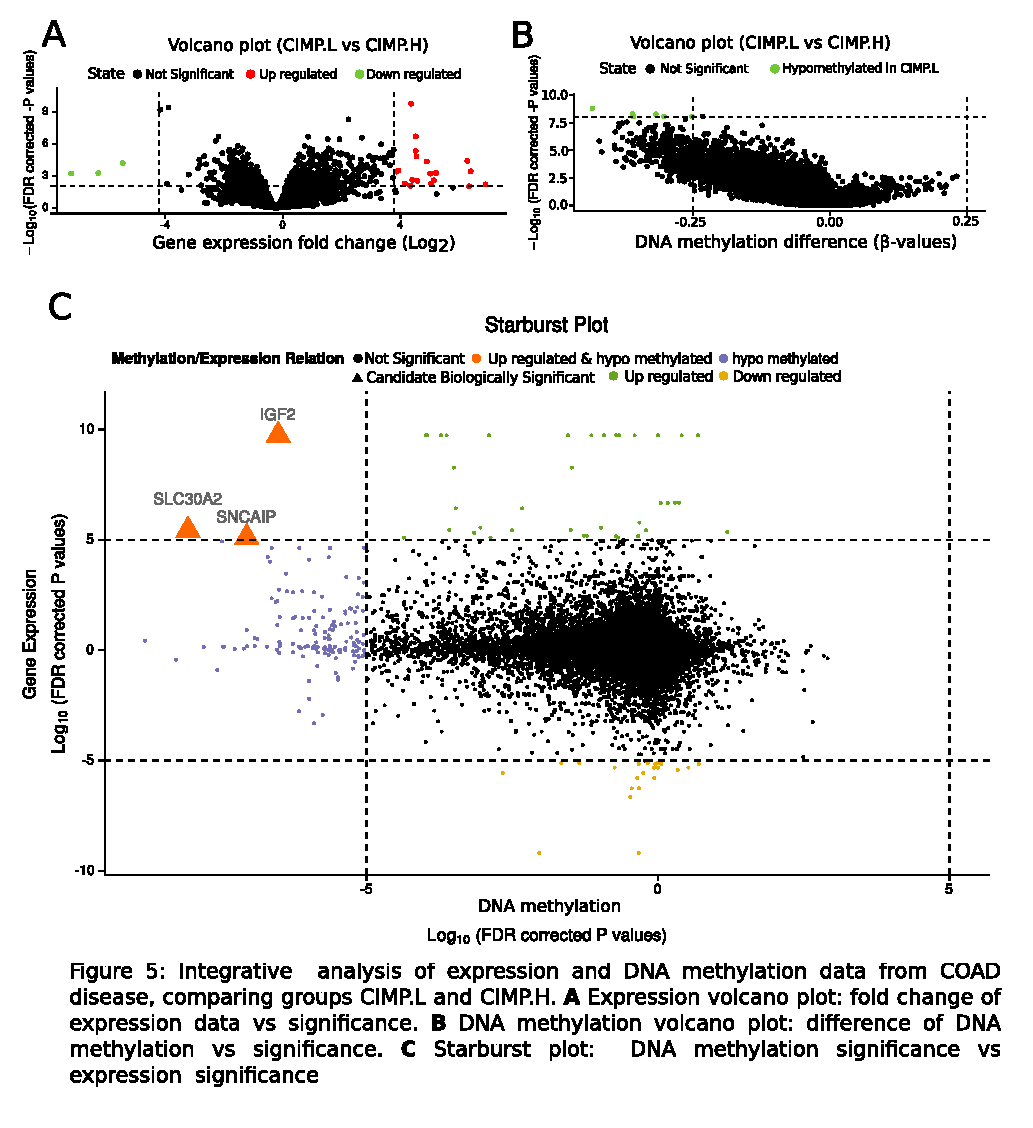
\includegraphics[width=.9\linewidth]{images/case3_improved2.pdf}

\caption{Integrative analysis of expression and DNA methylation from COAD disease}
\label{fig:workflow}
\end{figure*}

\newpage



\section{TCGAbiolinksGUI: A graphical user interface to analyze GDC cancer molecular and clinical data}

The National Cancer Institute's (NCI) Genomic Data Commons (GDC), a data sharing platform that promotes precision medicine in oncology, provides a rich resource of molecular and clinical data of  almost 13,000 tumor patient samples across 38 different cancer types and subtypes. The platform includes data from The Cancer Genome Atlas (TCGA) and Therapeutically Applicable Research to Generate Effective Treatments (TARGET). The data, which is publicly available, have been utilized by researchers to make novel discoveries and/or validate important findings. To enhance these findings, several important bioinformatics tools to harness genomics cancer data were developed, many of them belonging to the Bioconductor project \cite{gentleman2004bioconductor}. Among those tools is our tool TCGAbiolinks \cite{TCGAbiolinks}, which was developed to facilitate the analysis of TCGA data by incorporating the query, download and processing steps within the Bioconductor project \cite{gentleman2004bioconductor}. This tool allows users to integrate TCGA data with Bioconductor packages thus harnessing a wealth of statistical methodologies for biologically derived data. In addition, it provides integrative methodologies to perform several important downstream analyses, such as DNA methylation and Gene expression integration. A full detailed comparison between TCGAbiolinks and other bioinformatics tools to analyze TCGA data was previously detailed in our report in which we highlight key advantages of using TCGAbiolinks  \cite{TCGAbiolinks}. Although TCGAbiolinks is a suitable R package for most data analysts with a strong knowledge and familiarity with R specifically those who can comfortably write strings of common R commands, we developed TCGAbiolinksGUI to enable user access to the methodologies offered in TCGAbiolinks and to give users the flexibility of point-and-click style analysis without the need to enter specific arguments. TCGAbiolinksGUI takes in all the important features of TCGAbiolinks and offers a graphics user interface (GUI) thereby eliminating any need to familiarize TCGAbiolinks' key functions and arguments.  Tutorials via online documents and YouTube video instructions will assist end-users in taking full advantage of TCGAbiolinks.
Here we present TCGAbiolinksGUI an R/Bioconductor package which uses the R web application framework shiny \cite{shiny} to provide a GUI to process, query, download, and perform integrative analyses of TCGA data.

\subsection{Infrastructure}
The TCGAbiolinksGUI user interface was created using Shiny, a Web Application Framework for R, and uses several packages to provide advanced features that can enhance Shiny apps, such as shinyjs to add JavaScript actions \cite{shinyjs}, shinydashboard to add dashboards \cite{shinydashboard} and shinyFiles \cite{shinyFiles} to provide access to the server file system. 

The following R/Bioconductor packages are used as back-ends for the data retrieval and analysis: TCGAbiolinks \cite{TCGAbiolinks} which allows to search, download and prepare data from the NCI's Genomic Data Commons (GDC) data portal into an R object and perform several downstream analysis;  ELMER (Enhancer Linking by Methylation/Expression Relationship) \cite{yao2015inferring, ELMER2} which identifies DNA methylation changes in distal regulatory regions and correlate these signatures with the expression of nearby genes to identify transcriptional targets associated with cancer; ComplexHeatmap \cite{Gu20052016} to visualize data as oncoprint and heatmaps, pathview \cite{luo2013pathview} which offers pathway based data integration and visualization; and maftools \cite{Maftools} to analyze, visualize and summarize \sigla{MAF}{Mutation Annotation Format} files.


\subsection{Graphical user interface design}
The user interface has been divided into three main \sigla{GUI}{Graphical User Interface} menus. The first menu defines the acquisition of GDC data. The second defines the analysis steps which subdivides according to the molecular data types.  And the third is dedicated to harnessing integrative analyses. We present below a brief description of each menu and their features that can be accessed through a side panel (see figure \ref{fig:fig1}): 


\begin{itemize}
	\item \textbf{GDC Data:} Provides a guided approach to search for published molecular subtype information, clinical and molecular data. In addition, it downloads and processes the molecular data into an R object that can be used for further analysis.
	\item \textbf{Clinical analysis:} Performs survival analysis to quantify and test survival differences between two or more groups of patients and draws survival curves with the 'number at risk' table, the cumulative number of events table and the cumulative number of censored subjects table using the R/CRAN package survminer \cite{survminer}.
	\item \textbf{Epigenetic analysis:} Performs a Differentially methylated regions (DMR) analysis, visualizes the results through both volcano and heatmap plots, and visualizes the mean DNA methylation level by groups.
	\item \textbf{Transcriptomic analysis:} Performs a Differential Expression Analysis (DEA), and visualizes the results through both volcano and heatmap plots. For the genes found as upregulated or downregulated an enrichment analysis can be performed and pathway data can be integrated \cite{luo2013pathview}.
 	\item \textbf{Genomic analysis:} Visualize and summarize the mutations from MAF (Mutation Annotation Format) files through summary plots and oncoplots using the R/Bioconductor maftools package \cite{Gu20052016,Maftools}. % Cite complex heatmap
	\item \textbf{Integrative analysis:} Integrate the DMR and DEA results through a starburst plot. Also, using the DNA methylation data and the gene expression data the R/Bioconductor ELMER package can be used to discover functionally relevant genomic regions associated with cancer \cite{yao2015inferring, ELMER2}.
\end{itemize}

\subsection{Documentation}

We provide a guided tutorial for users via a vignette document which details each step and menu function available at \href{http://bit.do/TCGAbiolinksDocs}{http://bit.do/TCGAbiolinksDocs}, via online documents available at 
\href{http://bit.ly/TCGAbiolinks\_PDFTutorials}{http://bit.ly/TCGAbiolinks\_PDFTutorials}, and via YouTube video instructions showing step by step how each menu works available at \href{http://bit.ly/TCGAbiolinksGUI\_videoTutorials}{http://bit.ly/TCGAbiolinksGUI\_videoTutorials}, which assist end-users in taking full advantage of TCGAbiolinksGUI. A demonstration version of the tool is available at \href{http://tcgabiolinks.fmrp.usp.br:3838/}{http://tcgabiolinks.fmrp.usp.br:3838/}. Users are encouraged to report and file bug reports or feature requests via our GitHub repository \href{https://github.com/BioinformaticsFMRP/TCGAbiolinksGUI/issues}{BioinformaticsFMRP/TCGAbiolinksGUI/issues}. 

\subsection{Docker container}
To further simplify the usability and accessibility of our tool, we provide a docker image compatible with most popular operating system available at \\
\href{https://hub.docker.com/r/tiagochst/tcgabiolinksgui/}{https://hub.docker.com/r/tiagochst/tcgabiolinksgui/}. This file allows users to run TCGAbiolinksGUI without the need to install associated dependencies or configure system files, common steps required to run R installations and load R/Bioconductor packages. 



\section{Results and Discussion}
To provide the users with insights into the usability of our TCGAbiolinksGUI, 1) we compare with other bioinformatics tools currently published in the field; 2) we provide a use-case that allows users a step-by-step guide to analyzing their own cancer molecular data.

\subsection{Comparison of alternative software}

Web tools used for cancer data analysis might be classified into two broad groups. 
The first group only provides an interface to existing software analysis tools.
The Galaxy project (\href{https://galaxyproject.org/}{https://galaxyproject.org/}), which is an open, web-based platform for accessible, reproducible, and transparent computational biomedical research, is an example of such a tool that belongs to this group.
The other group is composed of exploratory tools mainly focused on the visualization of processed data and pre-computed results. The cBioPortal project \cite{gao2013integrative,cerami2012cbio}, by providing several visualizations for mining the TCGA data, is an example of a tool that falls within this classification.

 If one were to classify TCGAbiolinksGUI, it would belong to the first group. Compared to the Galaxy project, TCGAbiolinksGUI offers an open platform which improves the accessibility of R/Bioconductor packages, allowing users an advantage to integrate their features with existing Bioconductor packages without the need to go beyond the R/Shiny frameworks as a common feature from the Galaxy project, which requires the interface elements to be structured through XML files \cite{10.12688/f1000research.9821.1}. 
In addition, going beyond the R/Bioconductor environment requires more software dependencies which make the process to install Galaxy to use R/Bioconductor packages laborious.
On the other hand, compared to cBioPortal, TCGAbiolinksGUI allows users to perform deep integrative analysis by comparing different subtypes of data (i.e. performing an integrative analysis to compare breast cancer samples with a mutation on FOXA1 gene compared to wild-type samples using DNA methylation, gene expression, and motif enrichment analysis on genomic regions of interest). Although cBioPortal offers these features, it would require users to process each step independently and download outside of cBioPortal in order to perform such integrative analysis.


\section{Enhancer Linking by Methylation/Expression Relationships (ELMER)}

Motivated by our discovery of transcriptional enhancers in tissue DNA methylation data \cite{berman2012ng}, and subsequent approaches to linking these enhancers to transcriptional targets using a chromQTL approach \cite{aran2013dna} (reviewed in \citeonline{yao2015review}), we developed the the R/Bioconductor  \textit{ELMER} (Enhancer Linking by Methylation/Expression Relationships) package, a tool which infers regulatory element landscapes and transcription factor networks from cancer methylomes \cite{yao2015inferring}. 

This tool combined DNA methylation and gene expression data from human tissues to infer multi-level cis-regulatory networks through several steps which included the identification of distal enhancer probes with significantly altered DNA methylation levels in primary tumor tissues compared to normal tissues, followed by the identification of putative target genes, and a comprehensive gene regulatory network analysis which combined transcription factor motifs at the altered enhancers with TF expression to identify the underlying master regulators. This approach identified several known and unknown master regulators in TCGA data, such as \sigla{GATA3}{GATA-binding protein 3} and \sigla{FOXA1}{Forkhead box protein A1} in breast cancer, and \sigla{P63}{tumor protein p63} and \sigla{SOX2}{Sex determining region Y-box 2} in squamous cell lung carcinoma \cite{yao2015inferring,silva2016tcga}.

% Present \textit{ELMER}
Based on user feedback and a full review of the source code, we identified and implemented a number of software improvements, which are summarized in table \ref{tab:summary}: (i) The original package contained no standard data structure to handle multiple assays (DNA methylation, gene expression, and clinical data), which would be required for an integrative genomic data analysis. Recently, the Bioconductor team provided such a data structure through the \href{http://bioconductor.org/packages/MultiAssayExperiment/}{MultiAssayExperiment} package. (ii) All auxiliary databases (human TF list, classification of TF in families, gene annotation, DNA methylation annotation and motif occurrences within probe sites) used in the package were created and maintained manually, thereby making the upgrade process laborious; thus, we automated this process. (iii) The package was developed to analyze primary tumor tissue samples compared to normal tissues samples, thus not allowing arbitrary subgroups to be compared (for instance mutants vs. non-mutants, treated vs. untreated, etc.) (iv) Our original approach used known epigenomic markers for enhancers to constrain the genomic regions searched for differential methylation. However, this selection could limit our algorithm to identifying regulatory networks for tissue types that exist in the epigenomic databases; we found this constraint problematic, and thus now search \textit{all} distal regulatory regions without any such filter. (v) The function used to download data from The Cancer Genome Atlas (TCGA) data portal \cite{tomczak2015cancer} broke when the TCGA site was shutdown and its data transferred to The NCI's Genomic Data Commons (GDC) \cite{grossman2016toward}; we now have a more general data provider interface that supports GDC as the default provider. (vi) The package only supported data aligned to Genome Reference Consortium GRCh37 (hg19), and we now provide support for Genome Reference Consortium GRCh38 (hg38). (vii) There was no support to the recent HumanMethylationEPIC (EPIC) array \cite{epic}. In addition to the specific improvements listed above, we substantially re-wrote most of the code to be more efficient and maintainable,  also most of the output plots generated were improved.

\begin{table}[h!]
\centering
\caption{Main differences between ELMER old version (v.1) and the new version (v.2)}
\label{tab:summary}
\begin{tabular}{@{}p{3cm}p{5cm}p{6cm}@{}}
\toprule
\multicolumn{1}{c}{\textbf{Features}} & \multicolumn{1}{c}{\textbf{ELMER Version 1}} & \multicolumn{1}{c}{\textbf{ELMER Version 2}}   \\ \midrule
Primary data structure                   & mee object (custom data structure)                       & MAE object (Bioconductor data structure) \\
Auxiliary data                   & Manually created                       & Programmatically created \\
Number of human TFs                    & 1,982                                  & 1,987 (Uniprot database \cite{apweiler2004uniprot})                 \\
Number of TF motifs                   & 91                                     & 771  (HOCOMOCO v11 database \cite{kulakovskiy2016hocomoco})                 \\
TF classification                     & 78 families                            & 82 families and 331 subfamilies \newline(TFClass database \cite{wingender2013tfclass}) \\
Analysis performed            & Normal vs tumor samples & Group 1 vs group 2                       \\ 
Statistical grouping            & unsupervised only & unsupervised or supervised using labeled groups                       \\ 
TCGA data source                   & The Cancer Genome Atlas (TCGA) (not available)                   & The NCI's Genomic Data Commons (GDC)                                      \\
Genome of reference                   & GRCh37 (hg19)                          & GRCh37 (hg19)/GRCh38 (hg38)          \\
DNA methylation platforms             & HumanMethylation450                                   & HumanMethylationEPIC and HumanMethylation450                                \\
Graphical User interface (GUI)        & None                                   & TCGAbiolinksGUI                       \\
\bottomrule
\end{tabular}
\end{table}

Here, we present a new version of the R \textit{ELMER} package, which addresses all the issues described above. 
The new version of \textit{ELMER} (v2.0.0) is available as an R/Bioconductor package at \burl{https://github.com/tiagochst/ELMER}. And, the new version of \textit{ELMER.data} (v2.0.0), which provides auxiliary data required to perform the analysis, is available at 
\burl{https://github.com/tiagochst/ELMER.data}. 

\subsection*{Implementation}

Here we describe each of following analysis steps shown in figure \ref{fig:elmerworkflow}. For more details, please also check the original ELMER paper \cite{yao2015inferring}. 
\begin{itemize}
    \item Organize data as a \textit{MultiAssayExperiment} object
	\item Identify distal probes with significantly different DNA methylation level when comparing two sample groups.
	\item Identify putative target genes for differentially methylated distal probes, using methylation vs. expression correlation
	\item Identify enriched motifs for each probe belonging to a significant probe-gene pair
	\item Identify master regulatory Transcription Factors (TF) whose expression associate with DNA methylation changes at multiple regulatory regions.
\end{itemize}

Organization of data as a \textit{MultiAssayExperiment} object

To facilitate the analysis of experiments and studies with multiple samples the Bioconductor team created the \href{http://bioconductor.org/packages/SummarizedExperiment/}{\textit{SummarizedExperiment}} class \cite{huber2015orchestrating}, a data structure able to store data and metadata for a single experiment but not for data spanning several experiments for the same sample. To overcome this problem, recently, the MultiAssay SIG (Special Interest Group) created the \href{http://bioconductor.org/packages/MultiAssayExperiment/}{MultiAssayExperiment class} \cite{mae2017} a data structure to manage and preprocess multiple assays for integrated genomic analysis. This data structure is now an input for all main functions of \href{https://github.com/tiagochst/ELMER}{\textit{ELMER}} and can be generated by the \textit{createMAE} function. 



To perform \textit{ELMER} analyses, we need to populate a \textit{MultiAssayExperiment} with a DNA methylation matrix or \textit{SummarizedExperiment} object from HM450K or EPIC platform; a gene expression matrix or SummarizedExperiment object for the same samples; a matrix mapping DNA methylation samples to gene expression samples; and a matrix with sample metadata (i.e. clinical data, molecular subtype, etc.). If TCGA data are used, the last two matrices will be automatically generated.
If using non-TCGA data, the matrix with sample metadata should be provided with at least a column with a patient identifier and another one identifying its group which will be used for analysis, if samples in the methylation and expression matrices are not ordered and with same names, a matrix mapping for each patient identifier their DNA methylation samples and their gene expression samples should be provided to the \textit{createMAE} function.
Based on the genome of reference selected, metadata for the DNA methylation probes, such as genomic coordinates, will be added from   \href{http://zwdzwd.github.io/InfiniumAnnotation}{\citeonline{zhou2016comprehensive}}; 
and metadata for gene expression and annotation is added from Ensembl database \cite{yates2015ensembl} using \href{http://bioconductor.org/packages/biomaRt/}{biomaRt}
\cite{durinck2009mapping}. 

\subsubsection*{Selecting distal probes} 
Probes from HumanMethylationEPIC (EPIC) array and Infinium HumanMethylation450 (HM450) array are removed from the analysis if they have either internal SNPs close to the $3'$ end of the probe; non-unique mapping to the bisulfite-converted genome; or off-target hybridization due to partial overlap with non-unique elements \cite{doi:10.1093/nar/gkw967}. This probe metadata information is
included in \href{https://github.com/tiagochst/ELMER.data}{\textit{ELMER.data}} package, populated from the source file at \url{http://zwdzwd.github.io/InfiniumAnnotation} \cite{doi:10.1093/nar/gkw967}.
To limit ELMER to the analysis of distal elements, probes located in regions of $\pm2 kb$ around transcription start sites (TSSs) were removed.

\subsubsection*{Identification of differentially methylated CpGs (DMCs)}

For each distal probe, samples of each group (group 1 and group 2) are ranked by their DNA methylation beta values, those samples in the lower quintile (20\% samples with the lowest methylation levels) of each group are used to identify if the probe is hypomethylated in group 1 compared to group 2, using an unpaired one-tailed t-test. The 20\% is a parameter to the \textit{diff.meth} function called \textit{minSubgroupFrac}. For the (ungrouped) cancer case, this is set to 20\% as in \citeonline{yao2015inferring}, because we typically wanted to be able to detect a specific molecular subtype among the tumor samples; these subtypes often make up only a minority of samples, and 20\% was chosen as a lower bound for the purposes of statistical power (high enough sample numbers to yield t-test p-values that could overcome multiple hypothesis corrections, yet low enough to be able to capture changes in individual molecular subtypes occurring in 20\% or more of the cases.) This number can be set arbitrarily as an input to the \textit{diff.meth} function and should be tuned based on sample sizes in individual studies. In the \textit{Supervised} mode, where the comparison groups are implicit in the sample set and labeled, the \textit{minSubgroupFrac} parameter is set to 100\%.  An example would be a cell culture experiment with 5 replicates of the untreated cell line, and another 5 replicates that include an experimental treatment.

To identify hypomethylated DMCs, a one-tailed t-test is used to rule out the null hypothesis: $\mu_{group1} \geq \mu_{group2}$, where $\mu_{group1}$ is the mean methylation within the lowest group 1 quintile (or another percentile as specified by the \textit{minSubgroupFrac} parameter) and $\mu_{group2}$ is the mean within the lowest group 2 quintile. Raw p-values are adjusted for multiple hypothesis testing using the Benjamini-Hochberg method \cite{benjamini1995controlling}, and probes are selected when they had adjusted p-value less than $0.01$ (which can be configured using the \textit{pvalue} parameter). For additional stringency, probes are only selected if the methylation difference: $\Delta = \mu_{group1} - \mu_{group2}$ was greater than $0.3$. The same method is used to identify hypermethylated DMCs, except we use the \textit{upper} quintile, and the opposite tail in the t-test is chosen.

\subsubsection*{Identification of putative target gene(s)} 

For each differentially methylated distal probe (DMC), the closest 10 upstream 
genes and the closest 10 downstream genes are tested for inverse correlation between 
methylation of the probe and expression of the gene (the number 10 can be changed using the \textit{numFlankingGenes} parameter). To select these genes, 
the probe-gene distance is defined as the distance from the probe to the transcription 
start site specified by the ENSEMBL gene level annotations \cite{yates2015ensembl} accessed via
the R/Bioconductor package \href{http://bioconductor.org/packages/biomaRt/}{biomaRt} \cite{durinck2009mapping,durinck2005biomart}. By choosing a constant number of genes to test for each probe, our goal is to avoid systematic false positives for probes in gene rich regions. This is especially important given the highly non-uniform gene density of mammalian genomes.
Thus, exactly 20 statistical tests were performed for each probe, as follows. 

For each probe-gene pair, the samples (all samples from both groups) are divided into two 
groups: the M group, which consisted of the upper methylation quintile (the 20\%
of samples with the highest methylation at the enhancer probe), and the U group, 
which consists of the lowest methylation quintile (the 20\% of samples with the 
lowest methylation.) The 20\% ile cutoff is a configurable parameter \textit{minSubgroupFrac} in the \textit{get.pair} function.
As with its usage in the \textit{diff.meth} function, the default value of 20\% is a balance, allowing for the identification of changes in a 
molecular subtype making up a minority (i.e. 20\%) of cases, while also yielding 
enough statistical power to make strong predictions. For larger sample sizes or other experimental designs, this could be set even lower.

For each candidate probe-gene pair, 
the Mann-Whitney U test is used to test the null hypothesis that overall gene 
expression in group M is greater than or equal than that in group U. 
This non-parametric test was used in order to minimize the effects 
of expression outliers, which can  occur across a very wide dynamic range. 
For each probe-gene pair tested, the raw p-value $P_r$ is corrected for multiple 
hypothesis using a permutation approach as follows.
The gene in the pair is held constant, and \textit{x} random methylation probes are 
chosen to perform the same one-tailed U test, generating a set of \textit{x} permutation
p-values $P_p$. We chose the x random probes only from among those that were 
"distal" (farther than $2kb$ from an annotated transcription start site), in order 
to draw these null-model probes from the same set as the probe being tested \cite{sham2014statistical}. 
An empirical p-value $P_e$ value was calculated using the following formula 
(which introduces a pseudo-count of 1):

$$P_e = \frac{num(P_p \leq P_r)+ 1}{x+1}$$

Notice that in the \textit{Supervised} mode, no additional filtering is necessary to ensure that the M and U group segregate by sample group labels.  The two sample groups are segregated by definition, since these probes were selected for their differential methylation, with the same directionality, between the two groups. 



\subsubsection*{Characterization of chromatin state context of enriched probes using FunciVar}

Unlike version 1 of \textit{ELMER}, we now consider \textit{all} distal probes in the identification of regulatory elements. DNA methylation is known to affect several different classes of distal chromatin state element, including active enhancers, poised enhancers, and insulators. In order to provide a functional interpretation of the regulatory elements identified by \textit{ELMER}, we perform a chromatin state enrichment analysis of the probes within significant probe-gene pairs, using the \textit{statePaintR} tools from the \burl{www.statehub.org} \cite{statepaintr}, along with our new FunciVar package \cite{funcivar}. Enrichment of the putative pairs within chromatin states is calculated against a background model that uses the distal probe set that the putative pairs are drawn from. 

\subsubsection*{Motif enrichment analysis}
In order to identify enriched motifs and potential upstream regulatory TFs, all probes with occurring in significant probe-gene pairs are combined for motif enrichment analysis. \sigla{HOMER}{Hypergeometric Optimization of Motif EnRichment} \cite{heinz2010simple} is used to find motif occurrences in a $\pm 250bp$ region around each probe, using HOCOMOCO (HOmo sapiens COmprehensive MOdel COllection) v11 \cite{kulakovskiy2016hocomoco}. Transcription factor (TF) binding models are available at \burl{http://hocomoco.autosome.ru/downloads} (using the HOMER specific format with threshold score levels corresponding to p-value $ \leq 1^{-4}$). 

For each probe set tested (i.e. the set of all probes occurring in significant probe-gene pairs), a motif enrichment Odds Ratio and a 95\% confidence interval are calculated using following formulas:
$$p = \frac{a}{a + b}$$
$$P = \frac{c}{c + d}$$
$$Odds Ration = \frac{\frac{p}{(1-p)}}{\frac{P}{1-P}}= \frac{p(1-P)}{P(1-p)}=\frac{ad}{bc}$$
$$SD = \sqrt{\frac{1}{a} + \frac{1}{b} + \frac{1}{c} + \frac{1}{d}}$$

where $a$ is the number of probes within the selected probe set that contains one 
or more motif occurrences; $b$ is the number of probes within the selected probe 
set that do not contain a motif occurrence; $c$ and $d$ are the same counts within 
the entire array probe set (drawn from the same set of distal-only probes using the same definition as the primary analysis). A probe set was considered significantly enriched 
for a particular motif if the 95\% confidence interval of the Odds Ratio was 
greater than $1.1$ (specified by option \textit{lower.OR}, $1.1$ is default), and the motif 
occurred at least 10 times (specified by option \textit{min.incidence}, $10$ is default) in 
the probe set. 

%\section*{Results} % Optional - only if novel data or analyses are included
%This section is only required if the paper includes novel data or analyses, and should be written as a traditional results section.

\subsubsection*{Identification of master regulator TFs}

When a group of enhancers is coordinately altered in a specific sample subset, this is often the result of an altered upstream \textit{master regulator} transcription factor in the gene regulatory network. \textit{ELMER} tries to identify such transcription factors corresponding to each of the TF binding motifs enriched from the previous analysis step.
For each enriched motif, \textit{ELMER} takes the average DNA methylation of all distal probes (in significant probe-gene pairs) that contain that motif occurrence (within a $\pm 250bp$ region) and compares this average DNA methylation to the expression of each gene annotated as a human TF.

A statistical test is performed for each motif-TF pair, as follows. All samples 
are divided into two groups: the M group, which consists 
of the 20\% of samples with the highest average methylation at all motif-adjacent
probes, and the U group, which consisted of the 20\%  of samples with the lowest 
methylation. This step is performed by the \textit{get.TFs} function, which takes \textit{minSubgroupFrac} as an input parameter, again with a default of 20\%.
For each candidate motif-TF pair, the Mann-Whitney U test is used to test 
the null hypothesis that overall gene expression in group M is greater or equal 
than that in group U. This non-parametric test was used in order to minimize the 
effects of expression outliers, which can occur across a very wide dynamic range. 
For each motif tested, this results in a raw p-value ($P_r$) for each of the human TFs.
All TFs are ranked by their $-log_{10}(Pr)$ values, and those falling within the top 5\% of 
this ranking were considered candidate upstream regulators. The best upstream 
TFs which are known to recognize to specific binding motif are automatically extracted as putative 
regulatory TFs, and rank ordered plots are created to visually inspect these relationships, as shown in the example below. Because the same motif can be recognized by many transcription factors of the same binding domain family, we define these relationships at both the family and subfamily classification level using the 
classifications from TFClass database \cite{wingender2013tfclass}. Use of this database is a major change from version 1 of ELMER, which used custom curations for DNA binding domain families. Use of the TFClass database is preferable because it is well curated and regularly updated to reflect new findings.



%\begin{landscape}
\tikzstyle{container} = [
    rectangle,
    draw,
    inner sep=0.2 cm,
    dashed
]
\tikzstyle{start} = [circle,
					 minimum size=2mm,
                     rounded corners=3mm,
					 very thick,
                     draw=green!50!black,
                     top color=green!50!black,
                     bottom color=green!50!black, 
                     text=white,
                     font=\tiny]

\tikzstyle{end} = [circle,
				  minimum size=2mm,
                  rounded corners=3mm,
                  very thick,draw=red!50!black, 
                  top color=red!50!black,
                  bottom color=red!50!black, 
                  text=white,
                  font=\tiny]

\tikzstyle{function} = [rectangle,
						minimum size=6mm,
                        rounded corners=3mm,
                        very thick,
                        draw=black!50, 
                        top color=white,
                        bottom color=white,
                        font=\itshape\footnotesize]

\tikzstyle{datain} = [
	rectangle, 
	rounded corners, 
    minimum width=3cm, 
    minimum height=0.5cm,
    text centered,
    font=\footnotesize, 
    draw=green!50!black, 
    fill=white, 
    text=black
]
                      
\tikzstyle{dataaux} = [
	rectangle, 
    rounded corners, 
    minimum width=3cm, 
    minimum height=0.5cm,
    text centered,
    font=\footnotesize,
    draw=orange, 
    fill=white, 
    text=black
]
                       
\tikzstyle{dataout} = [
	rectangle, 
	rounded corners, 
    minimum width=3cm, 
    minimum height=0.5cm,
    text centered,
    font=\footnotesize, 
    draw=blue, 
    fill=white, 
    text=black
]

% Pacakge labels
\tikzstyle{arrow} = [
	thick,
    ->,
    >=stealth,
    -latex',
    draw,
    rounded corners
]

\tikzstyle{labelelmer}=[
	rectangle,
    draw,
    fill=black!50!red,
    draw = black,
    minimum width=450pt,
    minimum height=1.5em,
    text=white,
    rotate = 90, 
    label={[rotate=90]center:\textcolor{white}{\textbf{ELMER package}}}
]

\tikzstyle{labeltcgabiolinks}=[
	rectangle,
	draw,
    fill=black!50!blue,
    draw = black,
    minimum width=420pt,
    minimum height=1.5em,
    text = green,
    rotate = 90, 
    label={[rotate=270]center:\textcolor{white}{\textbf{TCGAbiolinks/TCGAbiolinksGUI packages}}}
]


\tikzstyle{labelfuncivar}=[
	rectangle,
	draw,
    fill=black!20!orange,
    draw = black,
    xshift = -0.0cm,
    minimum width=480pt,
    minimum height=1.5em,
    text=white,
    rotate = 0, 
    label={[rotate=0]center:\textcolor{white}{\textbf{StateHub/StatePaintR/funcivar package}}}
]
\tikzstyle{labelgdc}=[
	rectangle,
	draw,
    fill=black!50!gray,
    draw = black,
    minimum width=167pt,
    minimum height=1.5em,
    text=white,
    yshift = 0.10cm,
    xshift = 0.1cm,
    rotate = 0, 
    label={[rotate=0]center:\textcolor{white}{\textbf{GDC database}}}
]
\tikzstyle{every annotation}=[fill=white, font=\sf \small, scale=0.5, text width=4cm, inner sep=2mm, text=black,draw = orange]


\begin{figure}[!ht]
\centering
  \resizebox{0.95\textwidth}{!}{%
\begin{tikzpicture}[node distance = 1.5cm, auto, shorten >=1pt,thick,font=\itshape\footnotesize]
\linespread{0.8}{
%\node (start) [start] {START};
\node (func1) [function, yshift = -0.5cm] {\textit{createMAE}};
\node [datain, right of=func1, yshift = 0.5cm, xshift = 2cm] (dna) {DNA methylation object};
\node [datain, right of=func1, yshift = -0.5cm, xshift = 2cm] (exp) {Gene expression object};
\node (out1) [dataout, below of=func1, yshift = -0.3cm,text width=3cm] {Multi Assay Experiment object};
\node (func2) [function, below of = out1] {get.diff.meth};
%\node (out2) [dataout, below of=func2, yshift = 0.3cm] {List of differently methylated probes};
\node (func3) [function, below of=func2] {GetNearGenes};
%\node (out3) [dataout, below of=func2, yshift = 0.3cm] {List of near genes for differently methylated probes};
\node (func4) [function, below of=func3] {get.pair};
%\node (out4) [dataout, below of=func4, yshift = 0.3cm] {List of pairs: differently expressed gene and differently methylated probes};
\node (func5) [function, below of=func4, yshift = -0.5cm] {get.enriched.motif};
%\node (out5) [dataout, below of=func5, yshift = 0.3cm] {List of enriched motifs};
\node (func6) [function, below of=func5] {get.TFs};
\node (func7) [function, below of=func6,yshift = -0.5cm] {TF.survival};
%\node (out5) [dataout, below of=func5, yshift = 0.3cm] {List of regulator};
\node [dataaux, left of=func5, xshift =-3cm] (elmerdata1) {Probes.motif};
%\node [dataaux, above of=elmerdata1] (enhancer) {enhancer};
\node [dataaux, left of=func6, yshift = 0.0cm, xshift =-3cm] (elmerdata2) {motif.relevant.TFs};
\node [dataaux, left of=func6, yshift = -1.0cm, xshift =-3cm] (elmerdata3) {human.TFs};
%\node (end) [end, below of=func7] {END};
\node (func8) [function, left of=func1,yshift = -3cm,xshift = -3cm] {get.feature.probe};
\node (probes) [datain, left of=func1,xshift = -3cm] {distal probes};
\node [dataaux, below of=func8] (tss) {ENSEMBL TSS};
\node [dataaux, below of=tss] (probesmetadata) {Probes metadata};


% funcvat
\node (funciVar) [function, below of=func7, xshift = 3cm, yshift = -1.4cm] {enrich.segments};
\node [dataaux, left of=funciVar,xshift = -2cm] (statehub) {Statehub tracks};
%\node [dataaux, left of=statehub,xshift = -2cm, yshift = 0.2cm] (encode) {ENCODE};
%\node [dataaux, left of=statehub,xshift = -2cm, yshift = -0.4cm] (roadmap) {ROADMAP};
%\node [dataaux, left of=statehub,xshift = -2cm, yshift = 0.8cm] (blueprint) {BLUEPRINT};
%\draw [arrow,dashed,draw=orange] (encode.east) -- (statehub.west);
%\draw [arrow,dashed,draw=orange] (roadmap.east) -- (statehub.west);
%\draw [arrow,dashed,draw=orange] (blueprint.east) -- (statehub.west);

\draw [arrow,dashed,draw=orange] (statehub.east) -- (funciVar.west);

\draw [arrow] (func4) -- ++(4.9,0) -- ++(0,-1) |- node {} (funciVar);

% Draw edges
%\path [arrow] (start) -- (func1);
\path [arrow,dashed,draw=green!50!black] (dna) |- (func1);
\path [arrow,dashed,draw=green!50!black] (exp) |- (func1);
\draw [arrow,dashed,draw=blue] (out1.west) -- ++(-.5,0) -- ++(0,-1) |- (func4.west);
\draw [arrow,dashed,draw=blue] (out1.west) -- ++(-.5,0) -- ++(0,-1) |- (func6.west);
\draw [arrow] (func1) -- (out1);
\draw [arrow] (out1) -- (func2);
\draw [arrow] (func2) -- node {} (func3);
\draw [arrow] (func3) -- (func4);
\draw [arrow] (func4) -- node {} (func5);
\draw [arrow] (func5) -- node {}(func6);
\draw [arrow] (func6) -- (func7);
%\draw [arrow] (func7) -- (end);
\draw [arrow,dashed,draw=orange] (elmerdata1) -- node {} (func5);
\draw [arrow,dashed,draw=orange] (elmerdata2.east) -- (func6.west);
\draw [arrow,dashed,draw=orange] (elmerdata3.east) -- ++(.5,0) -- ++(0,0.2) |- (func6.west);
%\draw [arrow,dashed,draw=orange] (enhancer.north) -- (func8.south);
\draw [arrow,dashed,draw=orange] (tss.north) -- (func8.south);
\draw [arrow,dashed,draw=orange] (probesmetadata.east) -- ++(.1,0) -- ++(0,0.2) |- (func8.east);
\path [arrow,dashed,draw=green!50!black] (probes) -- (func1);
\draw [arrow] (func8.north)  --  (probes);

% Containers
\node [container, 
       fit=(exp)(dna)(func1)(probes), 
       label={[font=\scriptsize,anchor=east] west:Data input}]
       (container1){};
\node [container, 
	   fit=(func2), 
       label={[font=\scriptsize,anchor=west,name=lfunc1] east:{\parbox[c]{4.0cm}{Identifying differentially\\ methylated probes}}}]
       (container2){};
\node [container, 
       fit=(func3)(func4), 
	   label={[font=\scriptsize,anchor=west,name=lfunc2] east:{\parbox[c]{4.0cm}{Identifying putative \\probe-gene pairs}}}]
       (container3){};
\node [container, 
 	   fit=(func5), 
       label={[font=\scriptsize,anchor=west] east:{\parbox[c]{4.0cm}{Motif enrichment\\ analysis}}}]
       (container4){};
\node [container, 
       fit=(func6), 
       label={[font=\scriptsize,anchor=west] south east:Identifying regulatory TFs}]
       (container5){};
\node [container, 
       fit=(elmerdata1)(elmerdata1), 
       label={[name=l1,font=\scriptsize,anchor=east] west:ELMER.data}]
       (container6){};
%\node[draw,text width=3cm, above of = elmerdata1]{ELMER.data};
\node [container, 
	   fit=(func8)(probesmetadata), 
	   label={[name=l3,font=\scriptsize,anchor=east] west:{\parbox[r]{2.0cm}{Select probes \\$\pm 2Kb$  distant \\ from TSS}}}]
       (container8){};

\node [container, 
       fit=(elmerdata2), 
       label={[name=l2,font=\scriptsize,anchor=east] west:TFClass database}]
       (container7){};
\node [container, 
	   fit=(elmerdata3), 
	   label={[name=l3,font=\scriptsize,anchor=east] west:Uniprot database}]
       (container8){};
\node [draw,  
       minimum height=450pt,
	   minimum width=450pt,
       fit=(l1)(exp)(dna)(elmerdata3)(l2)(lfunc1)(lfunc2)]
       (container9){};
\node at (container9.west) [labelelmer] {};
  
%------------------------------ TCGAbiolinks
\node (GDCprepare) [function, right of = func1, yshift =-1.3cm,xshift =8.8cm] {\textit{GDCprepare}};
\node (GDCdownload) [function, above of = GDCprepare,yshift =-0.4cm] {\textit{GDCdownload}};
\node (GDCquery) [function, above of = GDCdownload,yshift =-0.4cm] {\textit{GDCquery}};
\node (TCGAanalysesurvival) [function, right of = func7,xshift =7.8cm] {\textit{TCGAanalyse\_survival}};
\node (TCGAanalyzeEAcomplete) [function, right of = func4,yshift =0.4cm,xshift =7.8cm] {\textit{TCGAanalyze\_EAcomplete}};
\node (TCGAanalyzePathview) [function, right of = func4,yshift =-0.7cm,xshift =7.8cm] {\textit{TCGAanalyze\_Pathview}};
\node (TCGAvisualizeoncoprint) [function, right of = func4,yshift =-1.8cm,xshift =7.8cm] {\textit{TCGAvisualize\_oncoprint}};

\draw [arrow] (GDCquery) -- node {}(GDCdownload);
\draw [arrow] (GDCdownload) -- (GDCprepare);
\draw [arrow] (GDCprepare.west) -- ++(-0.3,0) -- ++(0,0.2) |- (dna.east);
\draw [arrow] (GDCprepare.west) -- ++(-0.3,0) -- ++(0,0.2) |- (exp.east);

\node (subtypeinfo) [dataaux, below of = GDCprepare,yshift =0.6cm] {Subtype information};
\node (molecularinfo) [dataaux, below of = subtypeinfo,yshift =0.6cm] {Molecular data};
\node (clinicalinfo) [dataaux,  below of = molecularinfo,yshift =0.6cm] {Clinical data};
\node (mafinfo) [dataaux, below of = clinicalinfo,yshift =0.6cm] {Mutation data};

\draw [arrow,dashed,draw=orange] (mafinfo.east) -- ++(0.5,0) -- ++(0,-0.2) |-    (TCGAvisualizeoncoprint.east);
\draw [arrow,dashed,draw=orange] (clinicalinfo.east)  -- ++(0.3,0) -- ++(0,0.2) |-   (GDCprepare.east);
\draw [arrow,dashed,draw=orange] (subtypeinfo.east)   -- ++(0.2,0) -- ++(0,0.2) |-   (GDCprepare.east);
\draw [arrow,dashed,draw=orange] (molecularinfo.east) -- ++(0.3,0) -- ++(0,0.2) |-  (GDCprepare.east);
\node [draw,  
       minimum height=420pt,
       minimum width=170pt, 
       xshift = 0.25cm,
       yshift = -0.25cm,
       fit=(TCGAanalyzeEAcomplete)(GDCquery)(TCGAanalysesurvival)(clinicalinfo)(subtypeinfo)](container10){};
\node at (container10.east) [labeltcgabiolinks] {};
\draw [latex'-latex',double] (TCGAanalysesurvival) --  (func7);
\draw [arrow] (func4.east)  -- ++(4.4,0) -- ++(0,0.2) |-  (TCGAanalyzeEAcomplete);
\draw [arrow] (func4.east)  -- ++(4.4,0) -- ++(0,-0.2) |-  (TCGAanalyzePathview);
\draw [arrow] (func4.east)  -- ++(4.4,0) -- ++(0,-0.2) |-  (TCGAvisualizeoncoprint);
\draw [arrow] (func6.east)  -|   (TCGAvisualizeoncoprint.south);
%------------------------------ 
\node [labelgdc, above of = GDCquery,xshift=-0.30cm,yshift=-0.05cm] (gdc) {};
\draw [latex'-latex',double] (GDCquery) --  (gdc.300);

\draw [draw,dashed] (gdc.188) |- (GDCdownload.west);
\draw [arrow,dashed] (gdc.188) |- (mafinfo.west);
\draw [arrow,dashed] (gdc.188) |- (clinicalinfo.west) ;
\draw [arrow,dashed] (gdc.188) |- (molecularinfo.west) ;
}

\tikzstyle{labelencode}=[
	rectangle,
	draw,
    fill=black!50!gray,
    draw = black,
    minimum width=150pt,
    minimum height=1.5em,
    text=white,
    yshift = 0.10cm,
    xshift = 0.1cm,
    rotate = 0, 
    label={[rotate=0]center:\textcolor{white}{\textbf{ENCODE database}}}
]
\tikzstyle{labelroadmap}=[
	rectangle,
	draw,
    fill=black!50!gray,
    draw = black,
    minimum width=150pt,
    minimum height=1.5em,
    text=white,
    yshift = 0.10cm,
    xshift = 0.1cm,
    rotate = 0, 
    label={[rotate=0]center:\textcolor{white}{\textbf{ROADMAP database}}}
]
\tikzstyle{labelblueprint}=[
	rectangle,
	draw,
    fill=black!50!gray,
    draw = black,
    minimum width=150pt,
    minimum height=1.5em,
    text=white,
    yshift = 0.10cm,
    xshift = 0.1cm,
    rotate = 0, 
    label={[rotate=0]center:\textcolor{white}{\textbf{BLUEPRINT database}}}
]

\node [draw,  
       minimum height=6.52em,
       minimum width=480pt, 
       xshift = 1.60cm,
       yshift = 0.05cm,
       fit=(funciVar)(funciVar)](containerFunciVar){};
\node at (containerFunciVar.south) [labelfuncivar] {};


\node [labelencode, right of = statehub,xshift=-8.20cm,yshift=-0.15cm] (encode) {};
\node [labelroadmap, below of = encode,xshift=-0.1cm,yshift=0.7cm] (roadmap) {};
\node [labelblueprint, above of = encode,yshift=-0.8cm,xshift=-0.1cm] (blueprint) {};
%\draw [latex'-latex',double] (encode.180) --  (containerFunciVar.0);
\draw [double,->] (encode.0) --  (statehub.180);
\draw [double,->] (roadmap.0) -- ++(1.4,0) |-   (statehub.180);
\draw [double,->] (blueprint.0) -- ++(1.4,0) |-  (statehub.180);
\end{tikzpicture}
  }%
  
  \caption[ELMER workflow]{ELMER workflow: ELMER receives as input a DNA methylation object, a gene expression object (a matrix or a SummarizedExperiment object) and a Genomic Ranges (GRanges) object with distal probes to be used as filter which can be retrieved using the \textit{get.feature.probe} function. The function \textit{createMAE}  will create a Multi Assay Experiment object keeping only samples that have both DNA methylation and gene expression data. Genes will be mapped to genomic position and annotated using ENSEMBL database \cite{doi:10.1093/database/baw093}, while for probes it will add annotation from \citeauthor{doi:10.1093/nar/gkw967} (\href{http://zwdzwd.github.io/InfiniumAnnotation}{http://zwdzwd.github.io/InfiniumAnnotation}) . This MAE object will be used as input to the next analysis functions. First, it identifies differentially methylated probes followed by the identification of their nearest genes (10 upstream and 10 downstream) through the  \textit{get.diff.meth} and  \textit{GetNearGenes} functions respectively. For each probe, it will verify if any of the nearby genes were affected by its change in the DNA methylation level and a list of  gene and probes pairs will be outputted from \textit{get.pair} function. For the probes in those pairs, it will search for enriched regulatory Transcription Factors motifs with the  \textit{get.enriched.motif} function. Finally, the  enriched motifs will be correlated with the level of the transcription factor through the \textit{get.TFs} function. In the figure green Boxes represents user input data, blue boxes represents output object, orange boxes represent auxiliary pre-computed data and gray boxes are functions.}
  \label{fig:elmerworkflow}
\end{figure}
%\end{landscape}
